\documentclass{article}
\usepackage{fullpage}
\usepackage{graphicx}

\title{CHREST User Guide \\ (version 4.0.0)}
\author{Peter Lane}

\begin{document}
\maketitle
\tableofcontents

\newpage
\section{Getting Started}

CHREST is a cognitive architecture covering processes of visual attention,
memory, categorisation and simple problem solving.  The CHREST software
provides a graphical interface for some common types of models, and can 
also be used as a library to develop more sophisticated experiments or
CHREST-based agents in a programming language of your choice.

This document introduces the CHREST software, its capabilities and typical 
uses. 

\subsection{Download}

CHREST can be downloaded from one of:

\begin{itemize}
\item {\tt http://chrest.info/software.html}  (most stable)
\item {\tt http://github.com/petercrlane/chrest} (latest developments and source)
\end{itemize}

\noindent After downloading {\tt chrest-NNN.zip} (where NNN refers to the
latest version number), unpack the file to obtain the {\tt chrest} folder.

The folder contains some documentation, including a copy of this user guide and
a manual, the {\tt chrest.jar} software, and a folder of examples, including
models written in different programming languages and some sample datasets.

\subsection{Run}

CHREST runs on the Java Virtual Machine, and requires version 6 or later of the 
Java Runtime Environment to be installed.

In most cases, CHREST can be run by double-clicking on the file {\tt chrest.jar}, 
which will launch the graphical shell described in the next section.

In some cases you will need to use {\tt start-chrest.bat} (on Windows) or 
{\tt start-chrest.sh} (on Linux or Apple) to ensure the Java run-time is correctly 
called.

If you have special memory requirements, you will also need to edit the number
after the flag {\tt -Mmx} in the {\tt start-chrest} script.  Alternatively, use
the standard ways to manage the Java Virtual Machine appropriate to your
platform.

\subsection{Technical Details}

Source code is available from {\tt http://github.com/petercrlane/chrest}.

\noindent The CHREST software has been written by Peter Lane, and is released
under the Open Works License ({\tt http://owl.apotheon.org}).


\section{Graphical Environment}

The graphical environment supports the development of simple models, and
provides facilities to drive experiments and view information on the resulting
model and performance.  The main frame the user sees provides a menu for the
`Data', from which a dataset may be opened.  When a dataset is opened, the main
part of the frame will contain a set of controls appropriate to that dataset;
examples follow below.  The other menu is for the `Model', providing access to
a view of the model and a dialog to change its properties.

Figure~\ref{model-view} shows the main components of the model's view.  The
current time of the model is shown in the top left corner; two scrollable boxes
for the short-term memories show the contents of the nodes referred to; and the
right-hand side shows the long-term memory network.  Various parts of the
display may be modified: the long-term memory's orientation and size, and
resizable bars let you alter the amount of each window that is occupied.  The
`View' menu provides an option to save the long-term memory image to a file.
You may open several view windows onto the same model, and they will all update
as the model changes.  This enables you to look at different parts of the
long-term memory or details of the short-term memory separately.

\begin{figure}
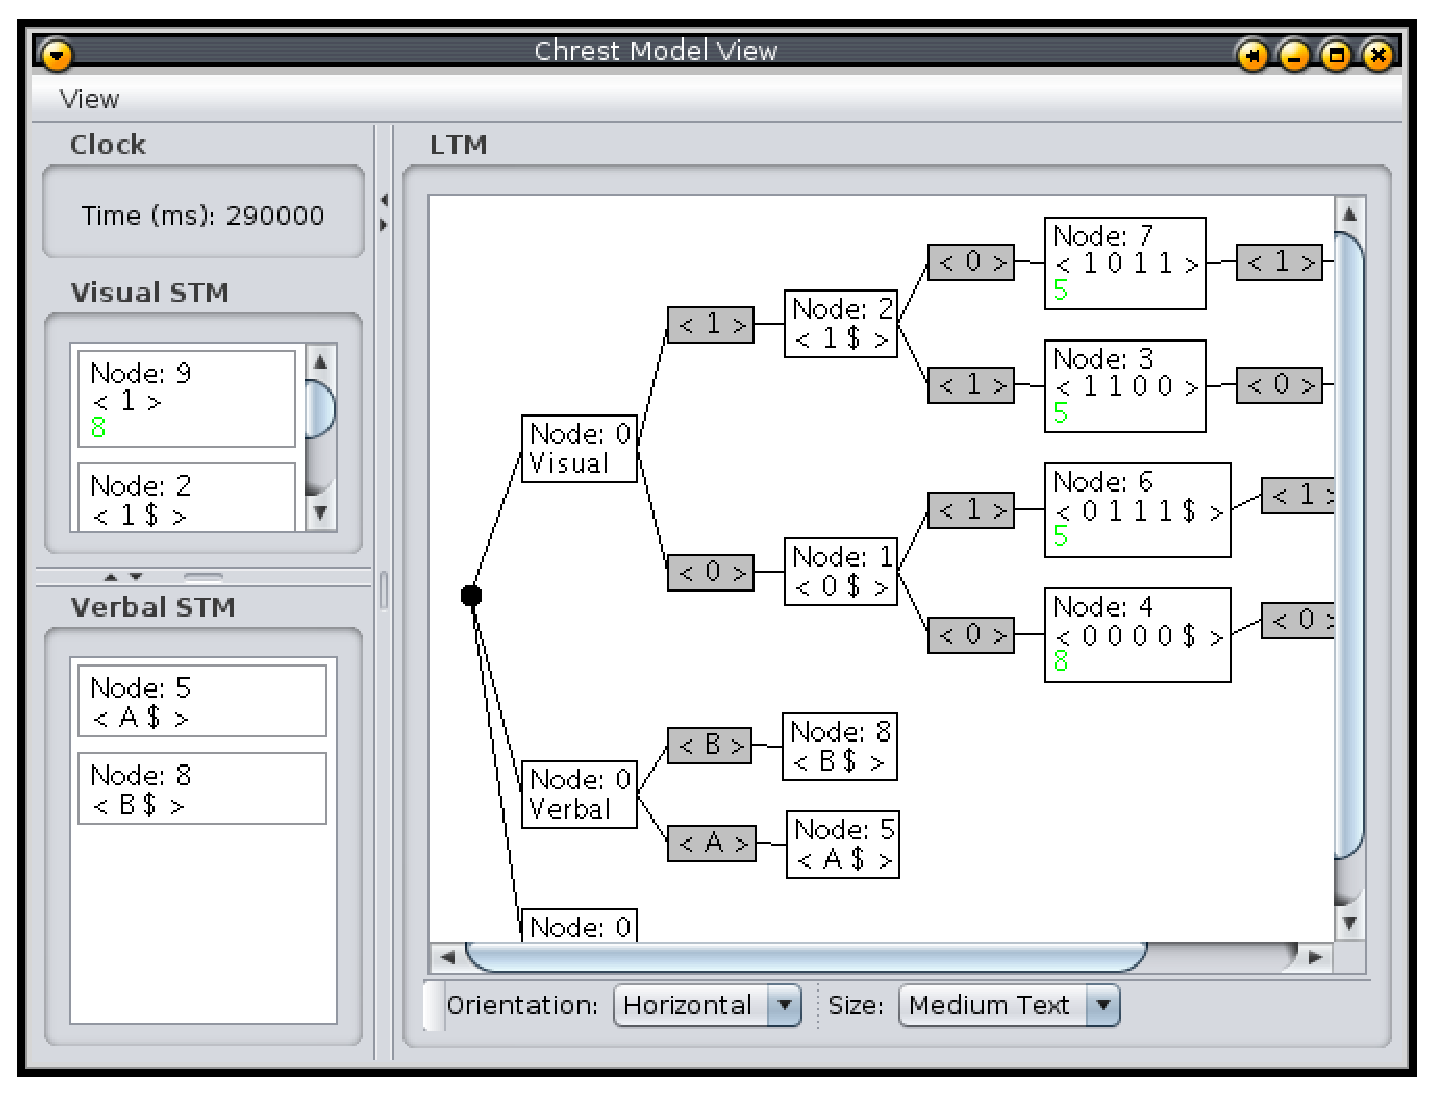
\includegraphics[width=4.0in]{images/model-view.eps}
\caption{View of model.  The LTM shows test links (in grey) and node images.
Each node has a unique number, and lateral links are shown by the coloured
numbers.}
\label{model-view}
\end{figure}

The Model/Properties menu option opens a dialog box, shown in
Figure~\ref{properties}, to view or change the parameters of the current CHREST
model.  Experimental data and definitions are provided through text files.  The
main types are described below.

\begin{figure}
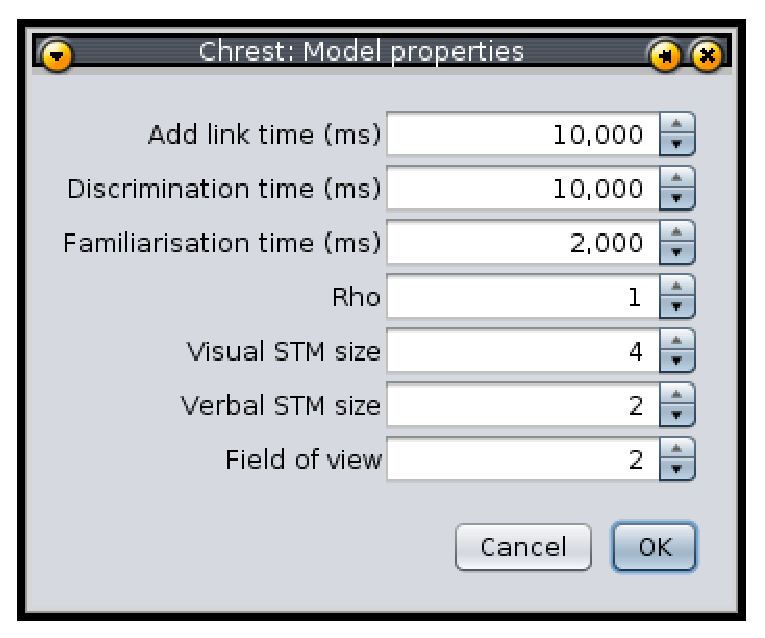
\includegraphics[width=3.0in]{images/properties.eps}
\caption{Dialog box to view or change parameters of a CHREST model.}
\label{properties}
\end{figure}

\subsection{Charts and Histograms}

The graphical environment provides a number of charts and histograms to display
information about the current model or experiment.  All these charts provide
functionality to zoom in/out of the display, alter the range of values
displayed, and to save as an image file.  This functionality is available in
most cases by right-clicking on the chart to bring up a menu.  Some useful
functions are described below:

\begin{enumerate}
\item Save image: right click on the display, and select `Save as...' from the menu.
\item Zoom in/out: right click on the display, and select zoom from the menu.
\item Change range: by dragging a rectangle over the area to see on the chart.
\item Precise range change: right click on the display, select `Properties...'.  Use the 
tab `Plot' and then (at the bottom of the display) `Range' for either `Domain axis' or `Range 
axis'.  Untick the `Autoadjust range' box, and enter the desired numbers.
\item Reset plot: right click on the display, and select `Autorange' and `Both axes'.
\end{enumerate}

\section{Supported Domains}

The graphical environment provides direct support for a number of typical 
domains and demonstrations.

\subsection{Learn and recognise}

The basic operations within CHREST are to learn about a new pattern and to
retrieve a familiar pattern when given a stimulus.  The learn-and-recognise
display allows the user to explore the basic learning mechanisms of the model.
The display is shown in Figure~\ref{learn-and-recognise}.  The list of patterns
is read from a data file.  The user highlights a pattern, and then uses one of
the buttons on the right either to `Learn' that pattern, or to `Recognise' that
pattern.  On clicking `Recognise' the display will show the image of the node
retrieved when the highlighted pattern is sorted through the network.  In this
case, the pattern {\tt $<$a b$>$} has been retrieved.  To speed up learning,
the user can use the `Learn all' button to learn each pattern once.  

\begin{figure}
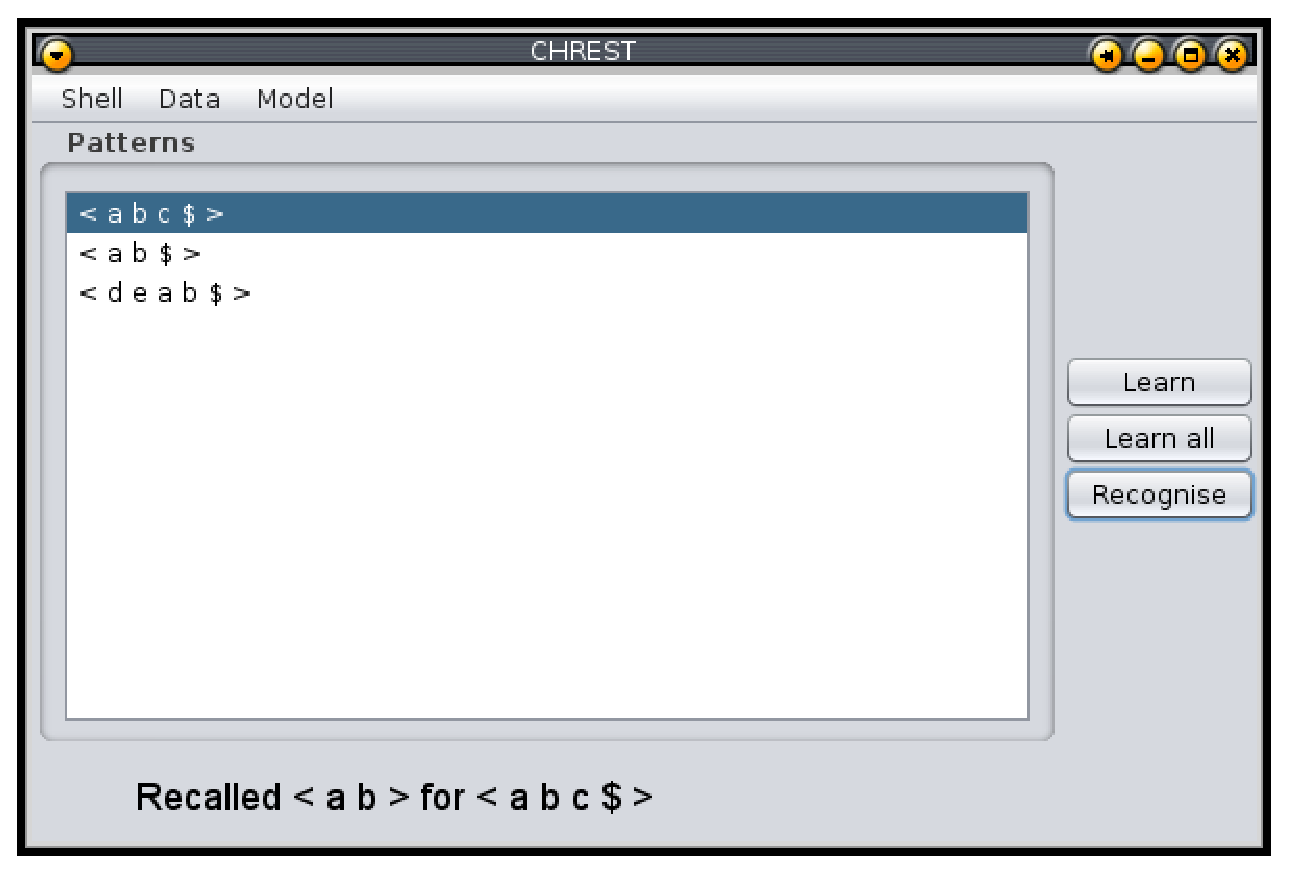
\includegraphics[width=4.0in]{images/learn-and-recognise.eps}
\caption{Learn and recognise display.}
\label{learn-and-recognise}
\end{figure}

No timing parameters are used in this system, and so it is ideal for observing
the basic learning mechanisms within CHREST by keeping a view of the model open
to one side.  An example data file is: 

\begin{verbatim}
recognise-and-learn 
a b c 
a b 
d e a b
\end{verbatim}

The file starts with the keyword `recognise-and-learn'.  Each pattern is on its
own line.  The atoms are separated by spaces.  The end marker is automatically
added to each pattern as it is defined, and so should not be part of the data
file.

\subsection{Paired associate learning}

This form of learning is about learning that one pattern is typically
associated with a second pattern: for example, seeing the word `dog' and
associating it with the word `cat'.  The verbal-learning paradigm was important
in psychological research when EPAM was being developed, and the core learning
mechanisms of EPAM and subsequently CHREST are based on the empirical support
from that time.  The experimental format supported in the interface is the
construction of a `subject protocol', which is a trial-by-trial list of all the
responses made by the human participant in the experiment.  For this kind of
task, the CHREST model forms sequence links between nodes of the same type in
its long-term memory; these links are shown in the model view as a blue number
inside the node, the number indicating the linked node.

\begin{figure}
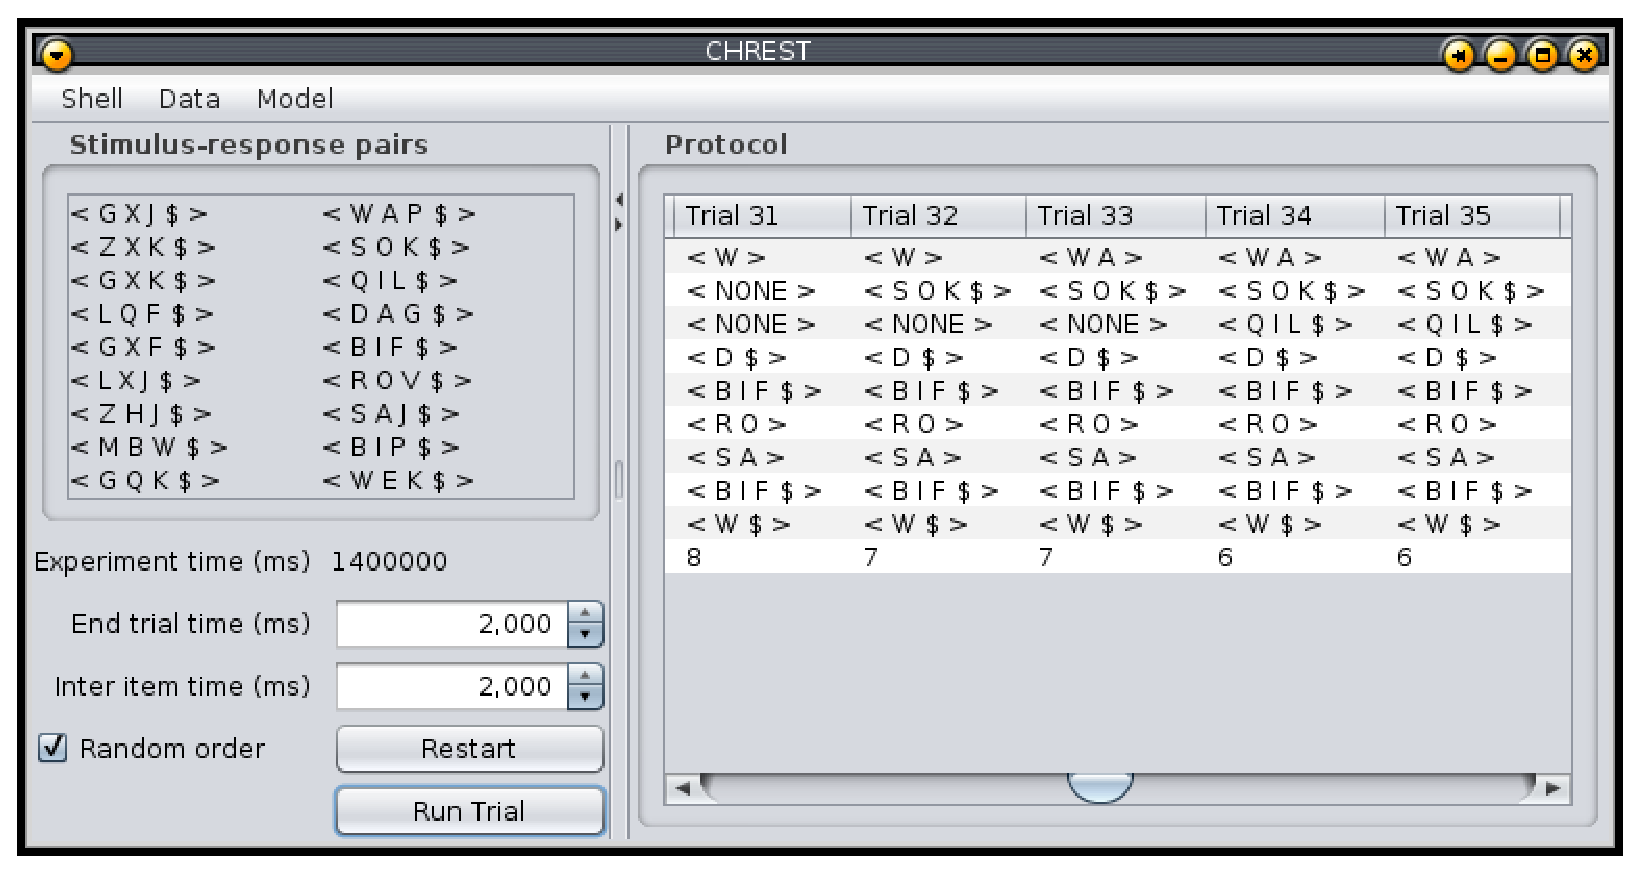
\includegraphics[width=4.0in]{images/paired-associate.eps}
\caption{Example of subject protocol for CHREST model of stimulus-response
experiment.}
\label{paired-associate}
\end{figure}

Figure~\ref{paired-associate} shows a typical view of the controls for this
type of experiment.  The controls on the left display the list of
stimulus-response pairs forming one set of data.  The times for which each item
in the list is presented, and also the time before the next trial is made, may
be altered.  The order of presentation may be as written or random, if the
checkbox is ticked.  The  `Run Trial' button will respect the given timings and
present each pattern in the list exactly once to the CHREST model.  The model's
response to each stimulus is provided in a new column in the protocol display
to the right of the display.  A count of the number of errors, responses that
are not identical to the target response, is provided below each column.  

There are two forms of the verbal-learning experiment.  The first is the
paired-associate experiment, where each pair is independent of the other pairs
in the list.  The second is the serial-anticipation task, where the idea is to
learn the sequence of patterns.  Both tasks can be controlled through the above
dialog (although for the second the `random order' option should not be used).
They have different definition files.  The serial-anticipation experiment is
simply a list of patterns, with each item in each pattern separated by a space.
The paired-associate experiment uses a list of pairs of patterns.  Each pair is
provided on its own line in the definition file, and the individual patterns of
each pair are separated by a colon.

\begin{minipage}{0.5\textwidth}
\begin{verbatim}
serial-anticipation 
D A G 
B I F 
G I H 
J A L 
M I Q 
P E L 
S U J
\end{verbatim} 
\end{minipage}
\begin{minipage}{0.5\textwidth}
\begin{verbatim}
paired-associate 
G X J : W A P 
Z X K : S O K 
G X K : Q I L 
L Q F : D A G 
G X F : B I F 
L X J : R O V 
Z H J : S A J 
M B W : B I P 
G Q K : W E K
\end{verbatim}
\end{minipage}

\subsection{Categorisation}

Categorisation is the process of assign labels to patterns.  We typically
handle categorisation in CHREST by providing the patterns to be named as visual
patterns, and the labels as verbal patterns.  Naming links are formed between
the two nodes as they co-occur during training; naming links are shown by
displaying the number of the linked node in green.

Figure~\ref{categorisation} depicts the categorisation experiment display.
This is very similar to that used in the verbal-learning above.  The second of
the two patterns is a verbal pattern, not a visual pattern.  Also, using the
tick boxes beside each pattern, the user can select which ones will form part
of the training data, and which only used for test.  The protocol is based on
the response of the model to each visual pattern, after each training cycle.

\begin{figure}
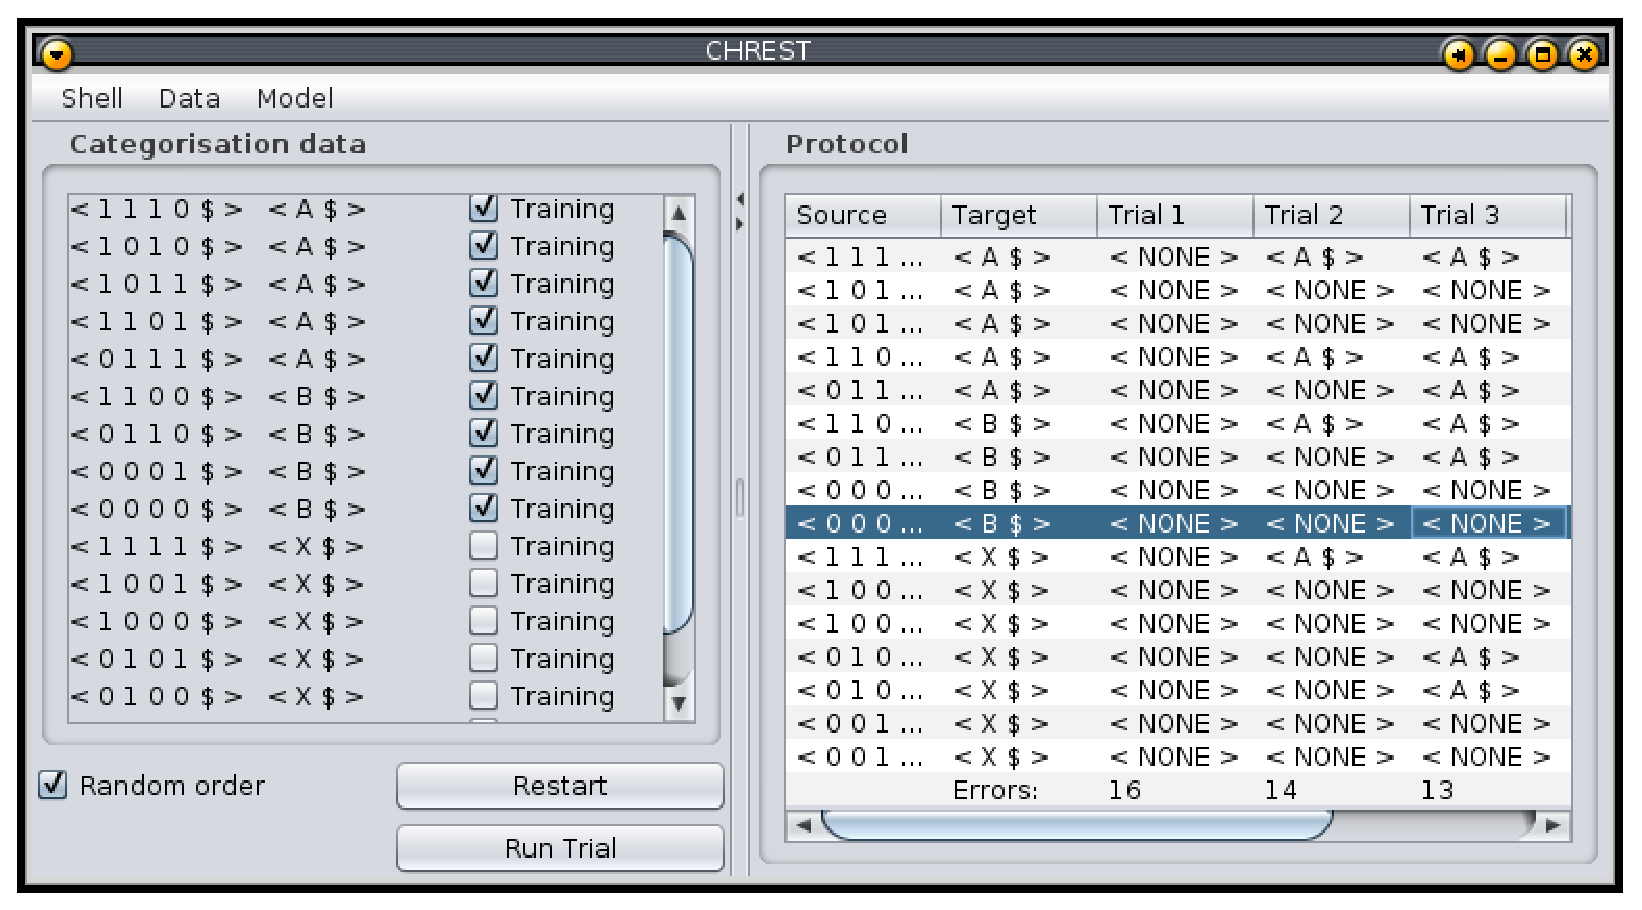
\includegraphics[width=\textwidth]{images/categorisation.eps}
\caption{Categorisation experiment display}
\label{categorisation}
\end{figure}

The data definition file for a categorisation experiment is very similar to
that for the paired-associate task, with the pattern to be named and its name
presented on the same line, separated by a colon:

\begin{verbatim}
categorisation 
1 1 1 0 : A 
1 0 1 0 : A 
1 0 1 1 : A 
1 1 0 1 : A 
0 1 1 1 : A 
1 1 0 0 : B 
0 1 1 0 : B 
0 0 0 1 : B 
0 0 0 0 : B 
1 1 1 1 : X 
1 0 0 1 : X 
1 0 0 0 : X 
0 1 0 1 : X 
0 1 0 0 : X 
0 0 1 1 : X 
0 0 1 0 : X 
\end{verbatim}

\subsection{Visual attention and recall}

CHREST has been used to model the visual attention processes and memory of
experts in domains such as chess.  The CHREST shell supports experiments in
chess and related domains. 

Figure~\ref{visual-search} shows the controls for training a model on a set of
scenes.  The drop-down box at the top allows selection of the domain: specific
domains tailor internal processes within CHREST and add heuristics, such as
following lines of attack/defence.  The aim of training is to create a CHREST
model of a given size.  The choice of maximum number of training cycles is to
place an upper limit on training times.  When the parameters are chosen, the
`train' button should be clicked, and the model will be created.  The graph and
progress bar will show progress towards the target number of chunks; the
process may be stopped by clicking the `stop' button.

\begin{figure}
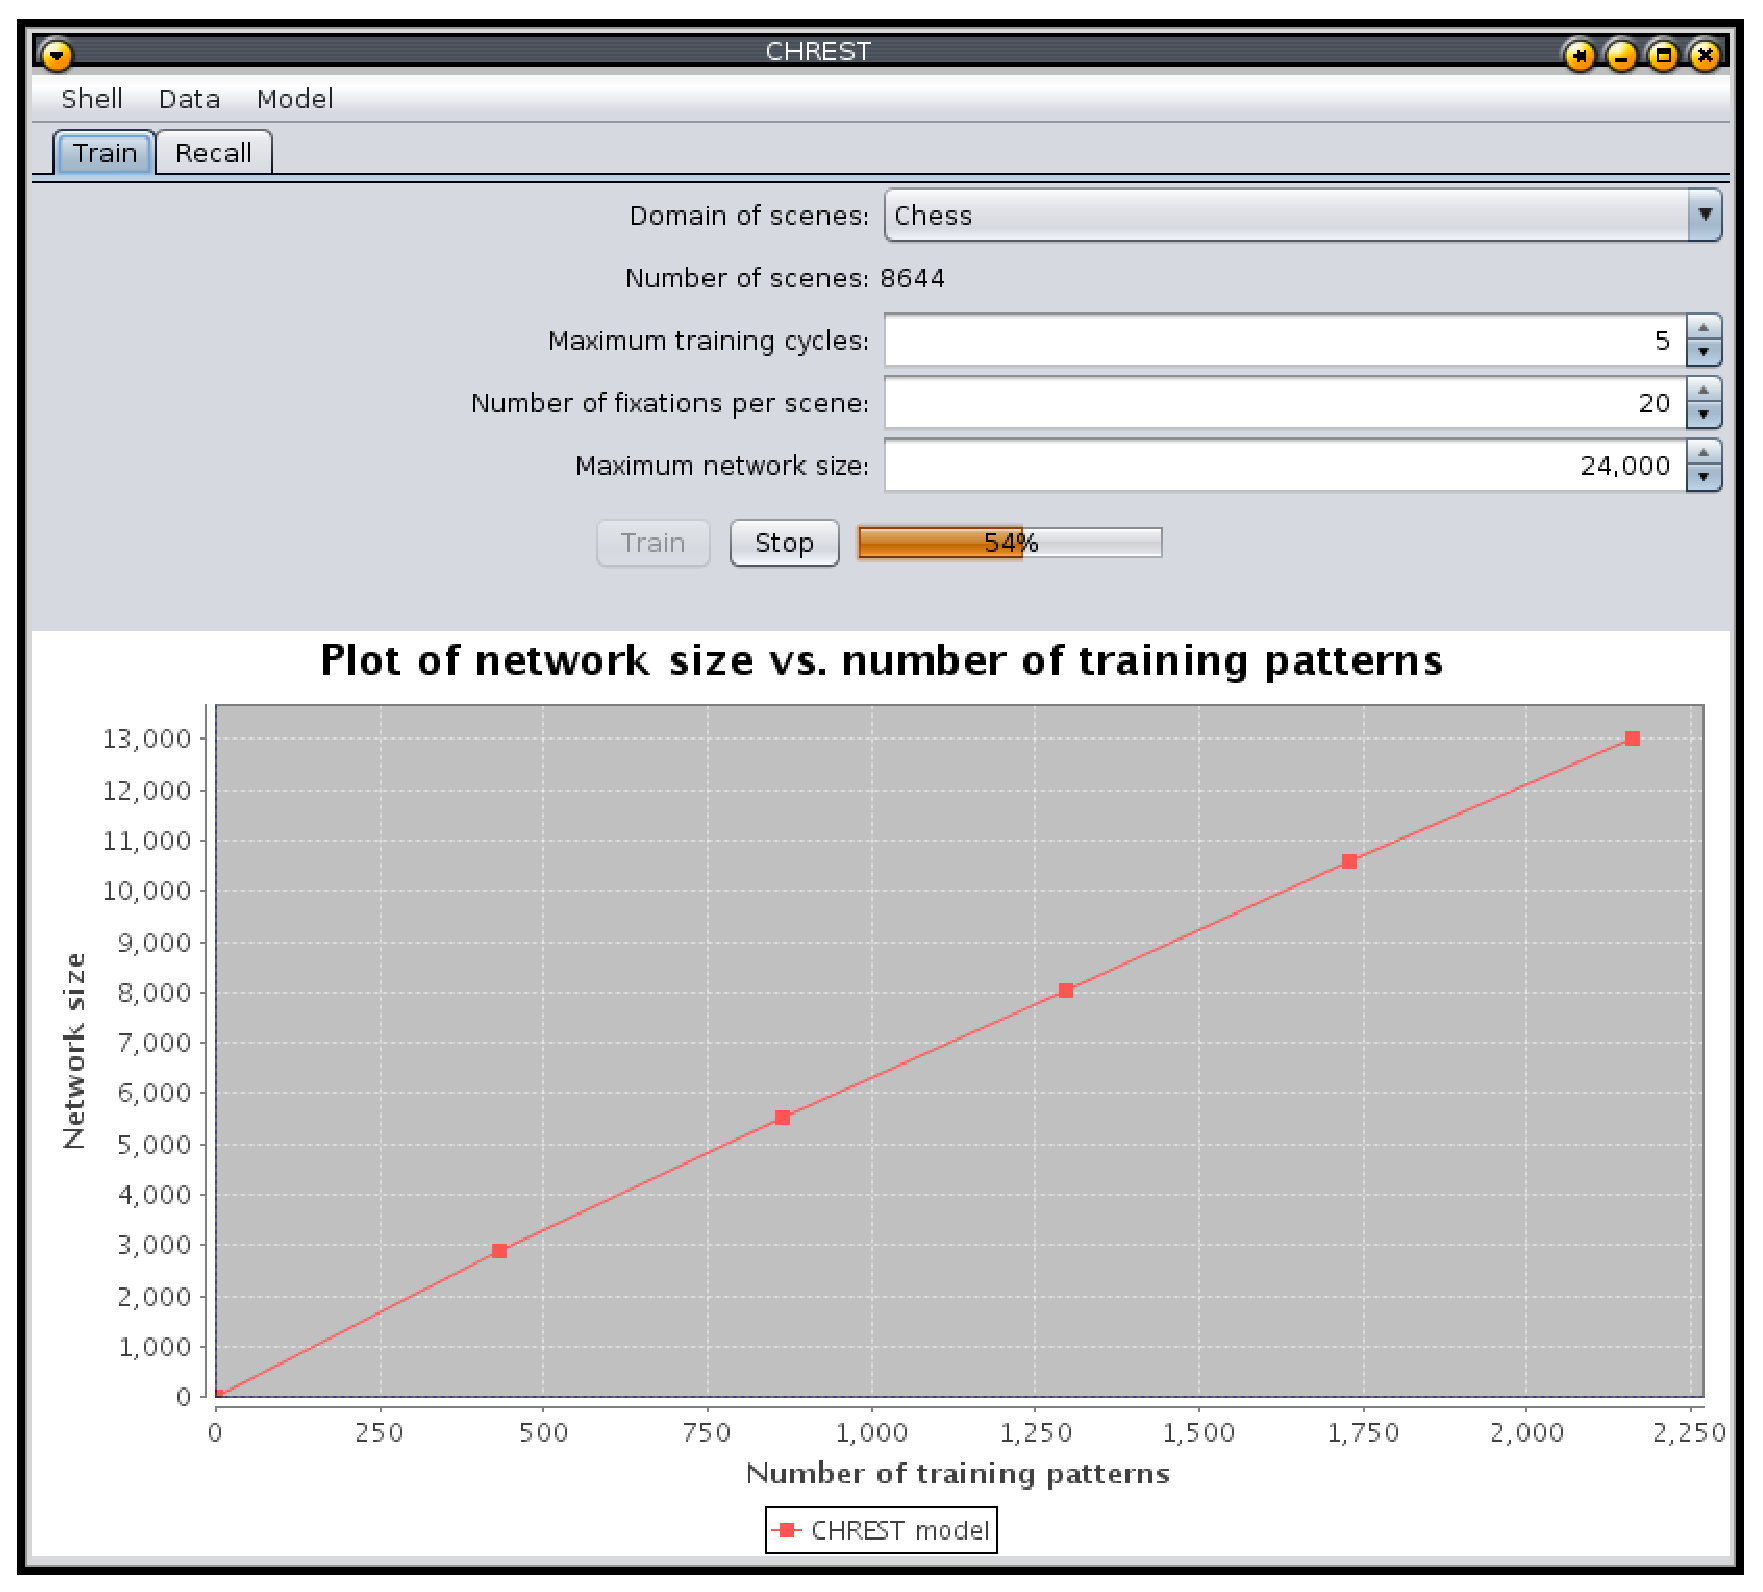
\includegraphics[width=\textwidth]{images/visual-search.eps}
\caption{Training a model from a set of scenes.}
\label{visual-search}
\end{figure}

Once trained, the model's recall performance can be tested.  It is possible to
use a separate set of files for recall by opening a new data file with the test
files; the model will not be changed.  Figure~\ref{recall} shows the screen on
the `recall' tab.  At the top, a drop-down list can be used to select the
target scene.  The button on the right will cause the model to scan the target
scene, and the recalled scene will be shown in the lower image.  Some
statistics on performance are also shown.

\begin{figure}
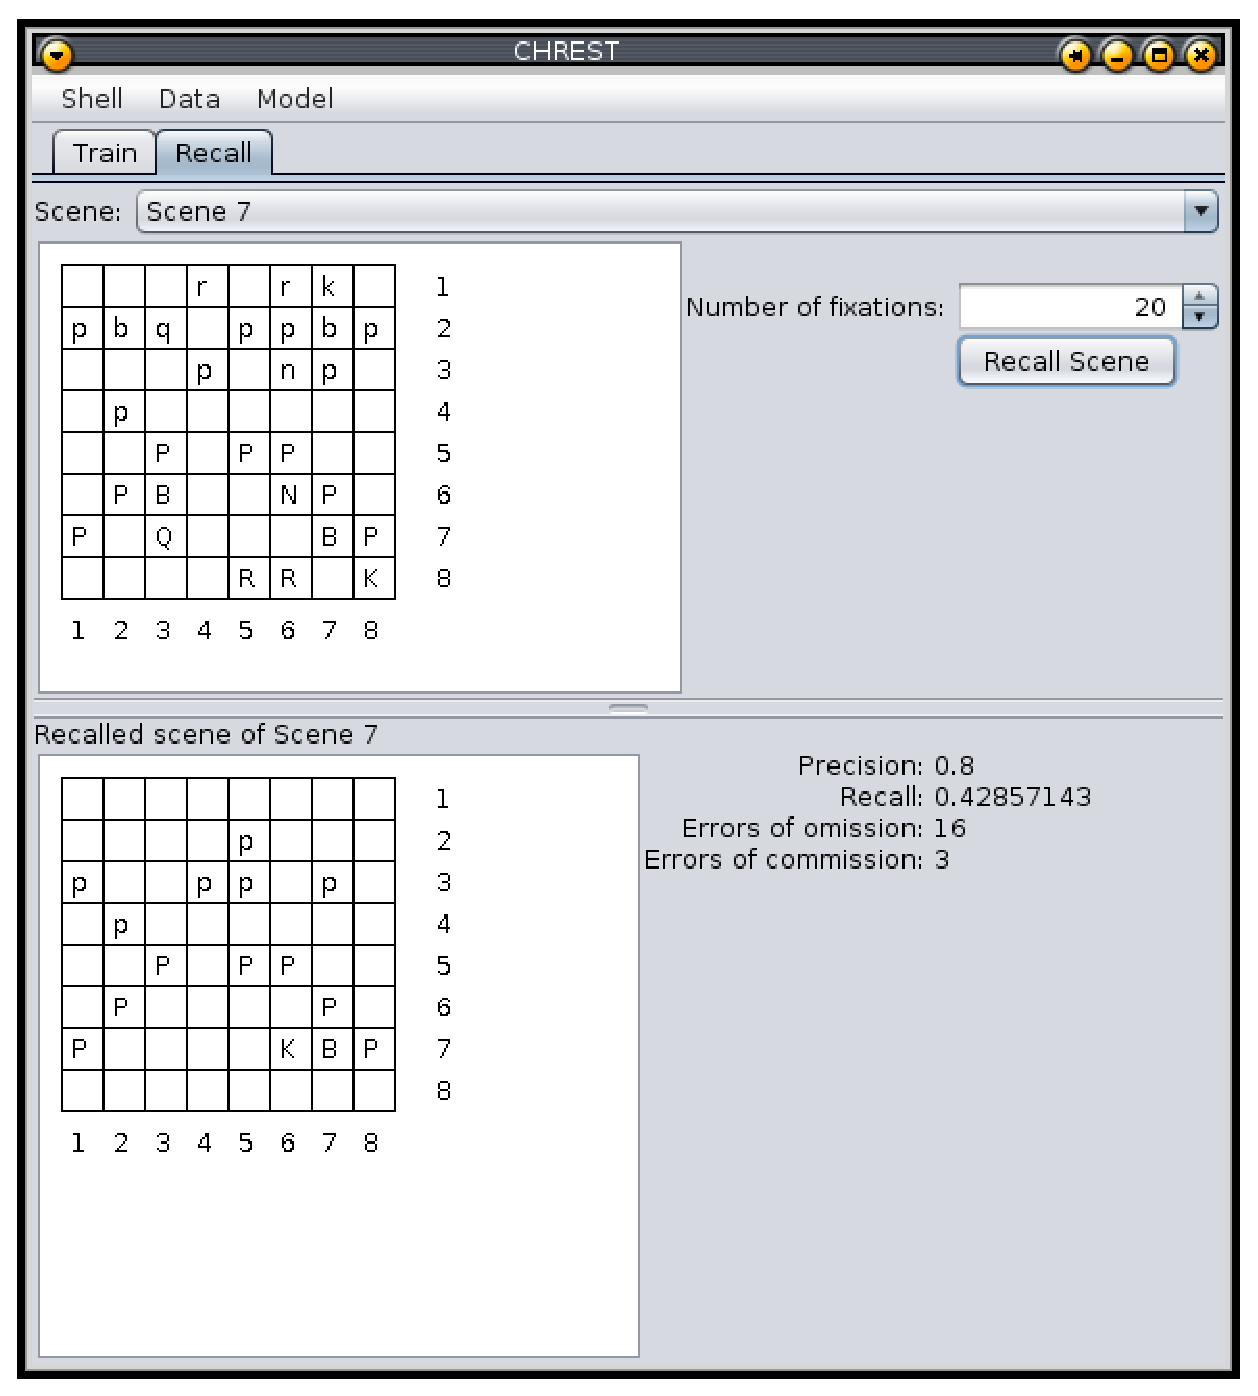
\includegraphics[width=\textwidth]{images/recall.eps}
\caption{Recall of a chess board.}
\label{recall}
\end{figure}

The data definition file for visual stimuli starts with the label
`visual-search', then the height and width of the patterns separated by a
space.  A blank line precedes the definition of the stimuli.  A full stop
indicates an empty space.  The following example defines two chess positions:

\begin{verbatim}
visual-search
8 8

..r.....
pb...pkp
.p.pq...
n..p..p.
...P....
Q..NP.P.
PP...PBP
.....RK.

r..q.rk.
.p...p..
p.n.p.p.
....Pnbp
P....B..
..NB....
.PP.Q.PP
R....R.K
\end{verbatim}

\newpage
\section{Scripting}

Although the graphical environment is useful for learning about CHREST, serious
modelling typically requires more control over the models and experimental
setup.  As CHREST runs on the Java virtual machine, any language which the Java
virtual machine supports can be used to develop CHREST-based models.  The
folder of examples includes scripts for a variety of languages including Lisp,
Ruby, Groovy (which is based on Java) and Clojure (which looks rather like
Lisp).  You can also use Java itself.\footnote{If you wish to learn a language
to begin writing models with CHREST, then Ruby is recommended, as more examples
are currently available and under active development.}

The javadoc documentation is provided for all classes within the chrest library; 
open the file `documentation/javadoc/index.html' in your browser.  

For most small projects, it is easy to create scripts using a reasonable editor
and running from the command line.  However, it is also possible to use a
development environment such as NetBeans or, for Lisp users, an appropriate
editor such as J or Emacs+SLIME.  For illustration, below are described some
environments for working with CHREST using Lisp, Ruby and Groovy.

\subsection{Development environment for Lisp}

The Lisp environment we recommend uses the java-based editor J and its related
lisp implementation ABCL.  The CHREST website provides a downloadable file
containing all the required files and further instructions on developing and
running CHREST models.

\subsection{Development environment for Ruby}

The following steps will let you develop models with jruby:

\begin{enumerate}
\item Download and install NetBeans, from {\tt http://netbeans.org/}
\item Install the ruby plugin
\item Create a new Ruby Project, using `File/New/Project'.  You will get a
dialog box similar to the one below.
\item After clicking `next' we need to tell NetBeans which ruby platform to
use.  You need to select a jruby platform, which should already be installed.
\item The final step in setting up the environment is to include the CHREST
library within the project. To do this , go to the `Java' option in the
Properties dialog box shown below. Select `Add JAR/Folder' and add the
{\tt chrest.jar} file to the classpath for this project. 
\item The only change you need to make to the ruby scripts is to remove the
line `require "chrest"'; this is taken care of by adding the jar file to the
project.
\end{enumerate}

\subsection{Development environment with Groovy}

The Groovy console provides an easy-to-use scripting environment for those
familiar with Groovy or the Java language.  Start the Groovy console, 
add the jar {\tt chrest.jar} to the classpath using the option under the `Scripts' 
menu, and then write code or load and run the examples.

\end{document}

